\section{Exploit}
In the following sections there are all the passages for the EternalBlue remote code execution.

\subsection{Small heap grooming}
The first step is making a small heap grooming with some secondary transactions.\\
The attacker sends the first transaction and some secondary transactions without the last one. In this way the server will allocate 
a srvnet buffer for each transaction in the memory.
\begin{figure}[ht!]
    \centering
      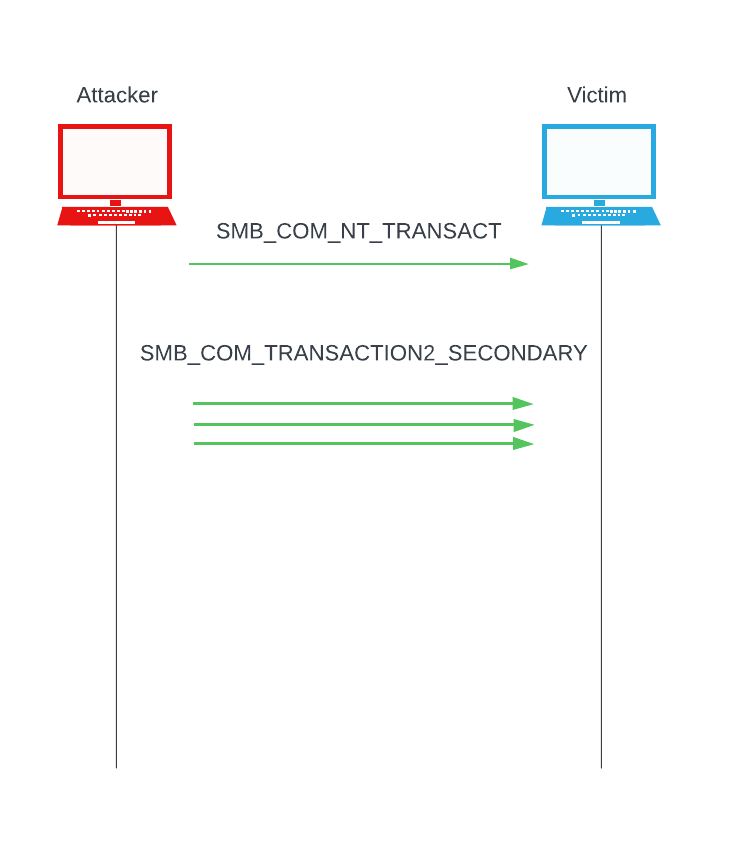
\includegraphics[scale=0.5]{images/exploit_1_comm.png}
      \caption{Small heap grooming - communications}
\end{figure}

\begin{figure}[ht!]
    \centering
      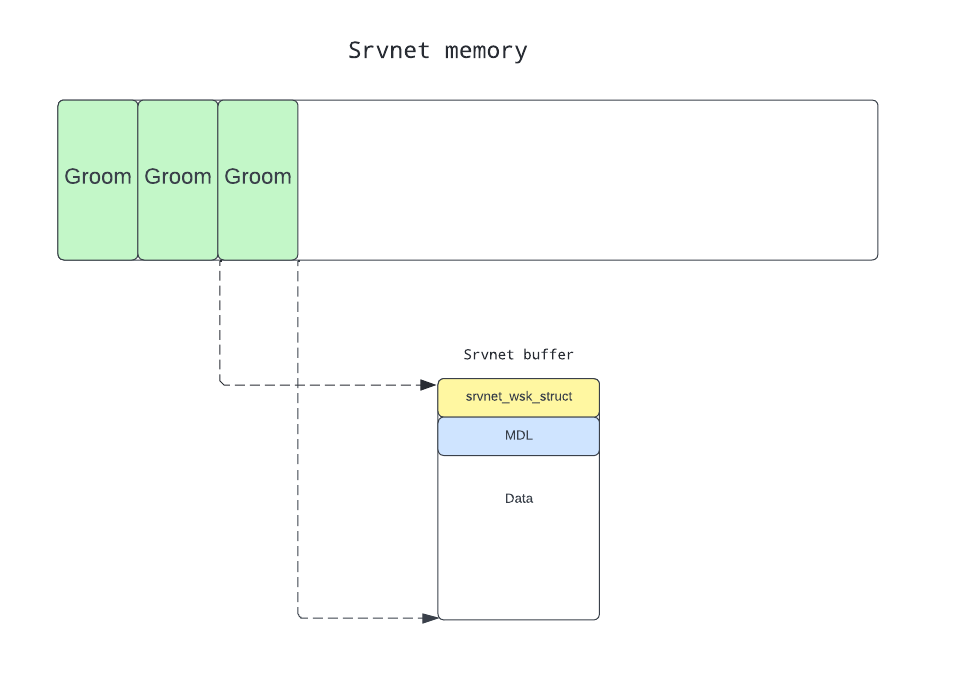
\includegraphics[scale=0.5]{images/exploit_1_buff.png}
      \caption{Small heap grooming - memory buffer}
\end{figure}


\clearpage
\subsection{Session setup allocation}
In this step we use the session setup bug explained in 3.3 to create a memory allocation with a specific size.\\
The size of the memory allocated will be the same of the future NT Buffer in order to do the remote heap allocation.\\

\begin{figure}[ht!]
    \centering
      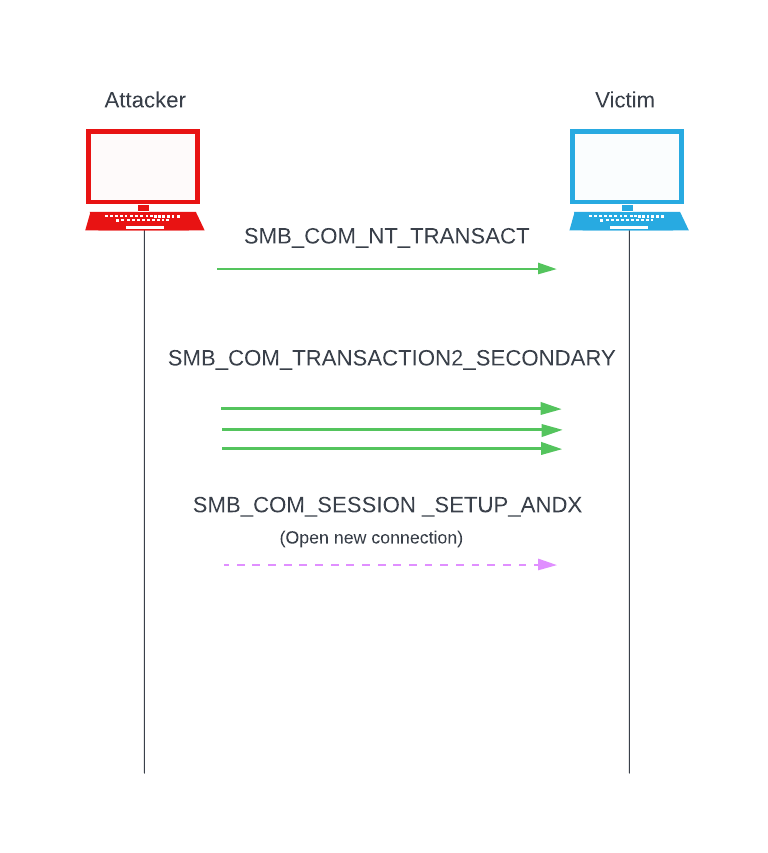
\includegraphics[scale=0.5]{images/exploit_2_comm.png}
      \caption{Session setup allocation - communications}
\end{figure}

\begin{figure}[ht!]
    \centering
      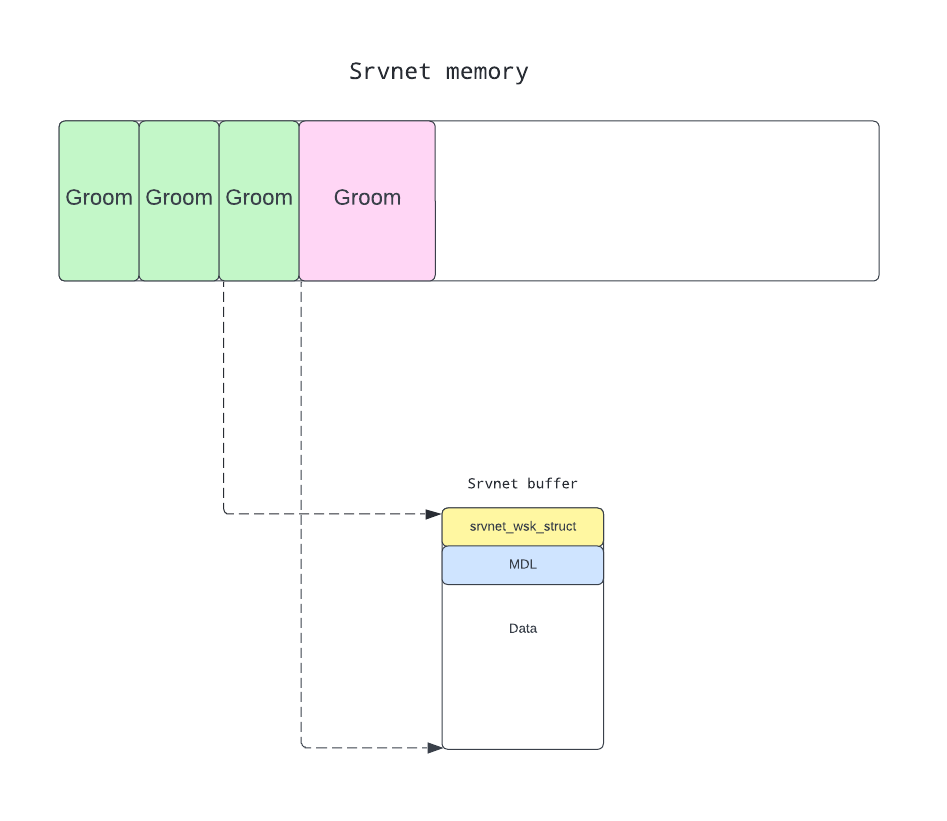
\includegraphics[scale=0.5]{images/exploit_2_buff.png}
      \caption{Session setup allocation - memory buffer}
\end{figure}

\clearpage
\subsection{Keep grooming}
In this step the attacker sends some secondary transactions to make the custom-sized memory contiguous to another srvnet buffer.

\begin{figure}[ht!]
    \centering
      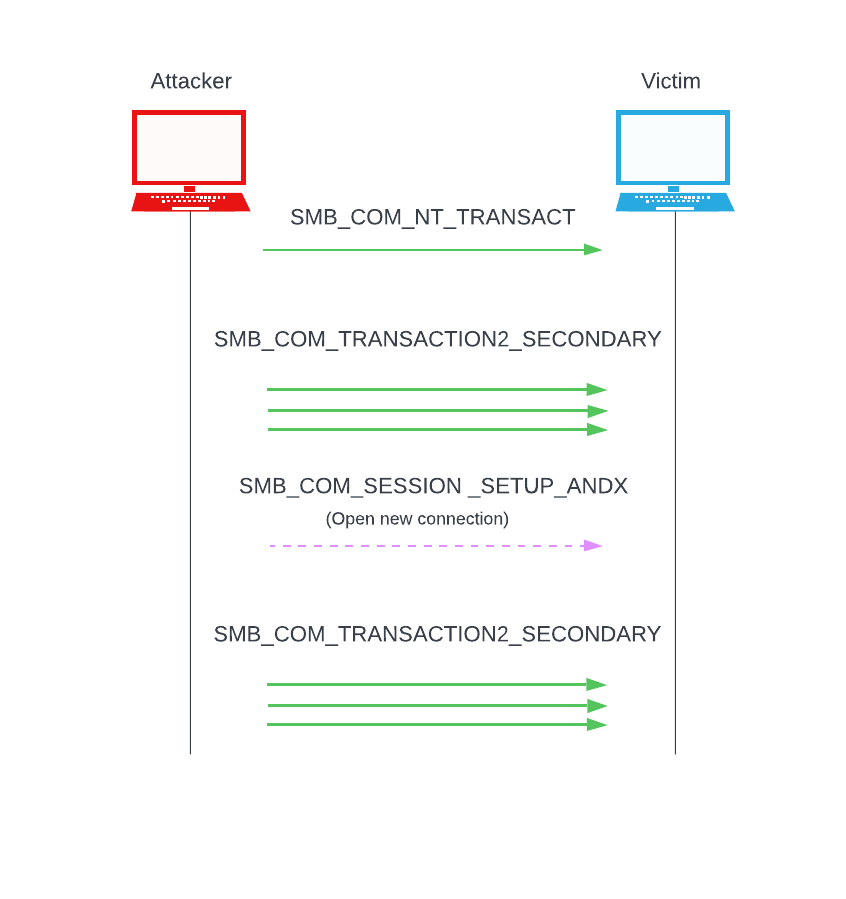
\includegraphics[scale=0.5]{images/exploit_3_comm.png}
      \caption{Keep grooming - communications}
\end{figure}

\begin{figure}[ht!]
    \centering
      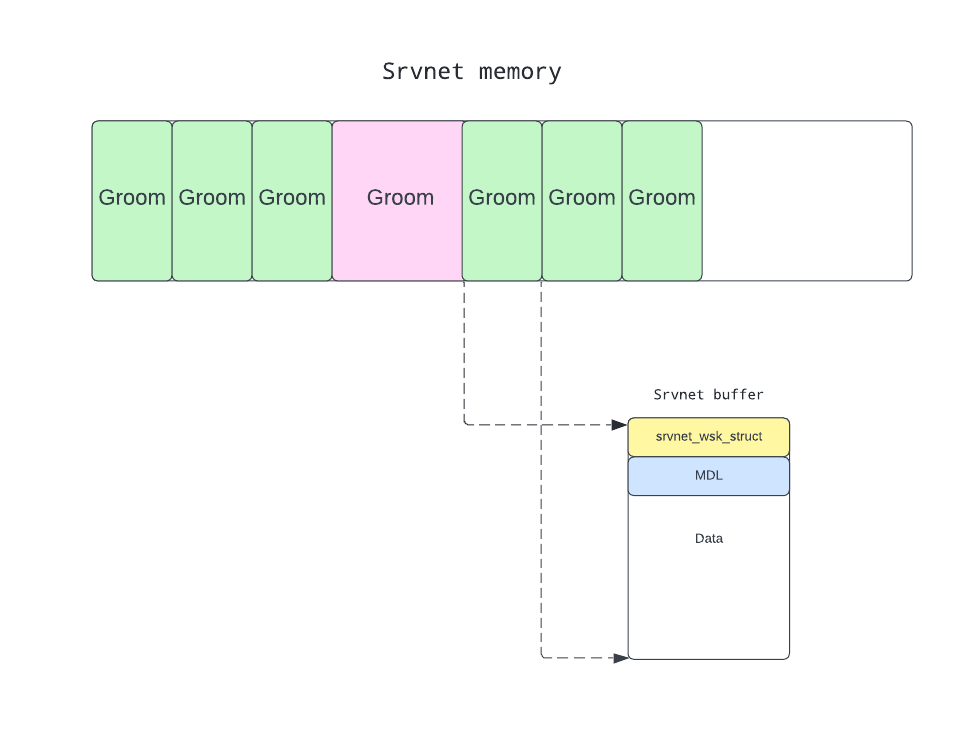
\includegraphics[scale=0.5]{images/exploit_3_buff.png}
      \caption{Keep grooming - memory buffer}
\end{figure}


\clearpage
\subsection{Creating the hole}
Now the attacker has to close the session opened in 6.2 in order to create a custom-sized hole in the heap memory.

\begin{figure}[ht!]
    \centering
      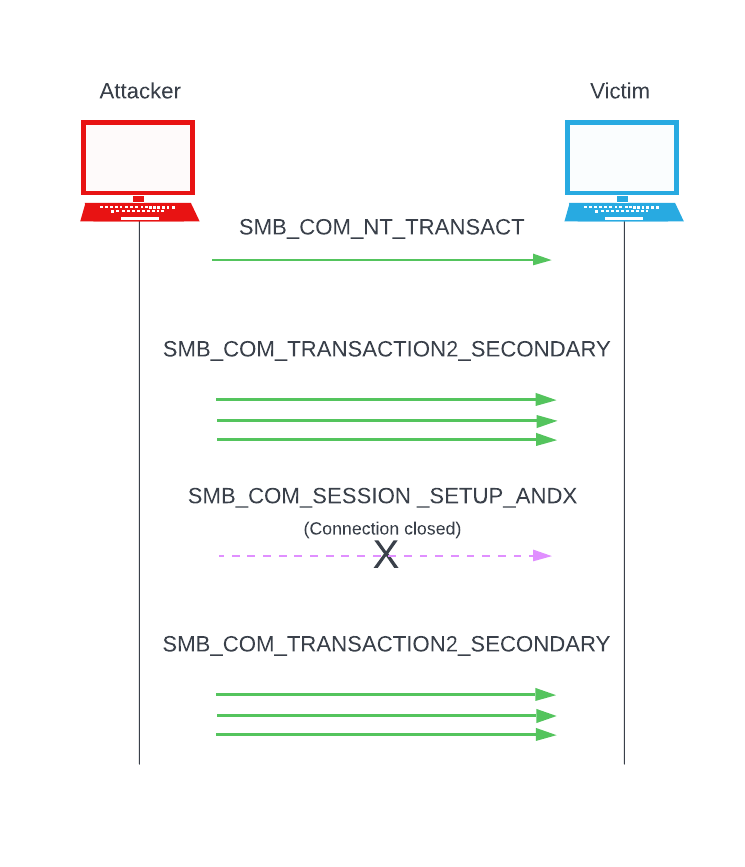
\includegraphics[scale=0.5]{images/exploit_4_comm.png}
      \caption{Creating the hole - communications}
\end{figure}

\begin{figure}[ht!]
    \centering
      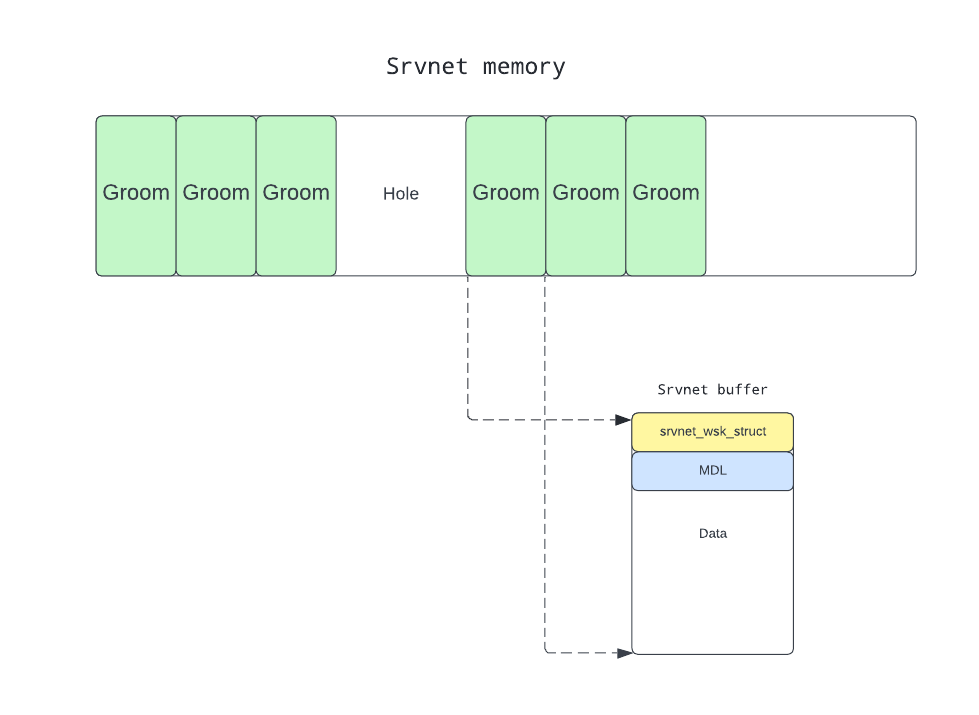
\includegraphics[scale=0.5]{images/exploit_4_buff.png}
      \caption{Creating the hole - memory buffer}
\end{figure}

\clearpage
\subsection{Buffer overflow}
Because of the grooming technique is very probable that the next transaction's buffer will be memorized in 
the hole that we have created in the previous step because it has the same size of the hole.\\
Now, the attacker can use the main bug explained in 3.1 to overflow the FEAList and overwrite the headers of the contiguous srvnet buffer.\\
In particular, he overwrites the pointers of the svrnet struct and the MDL in order that they point to the HAL's heap addresses.

\begin{figure}[ht!]
    \centering
      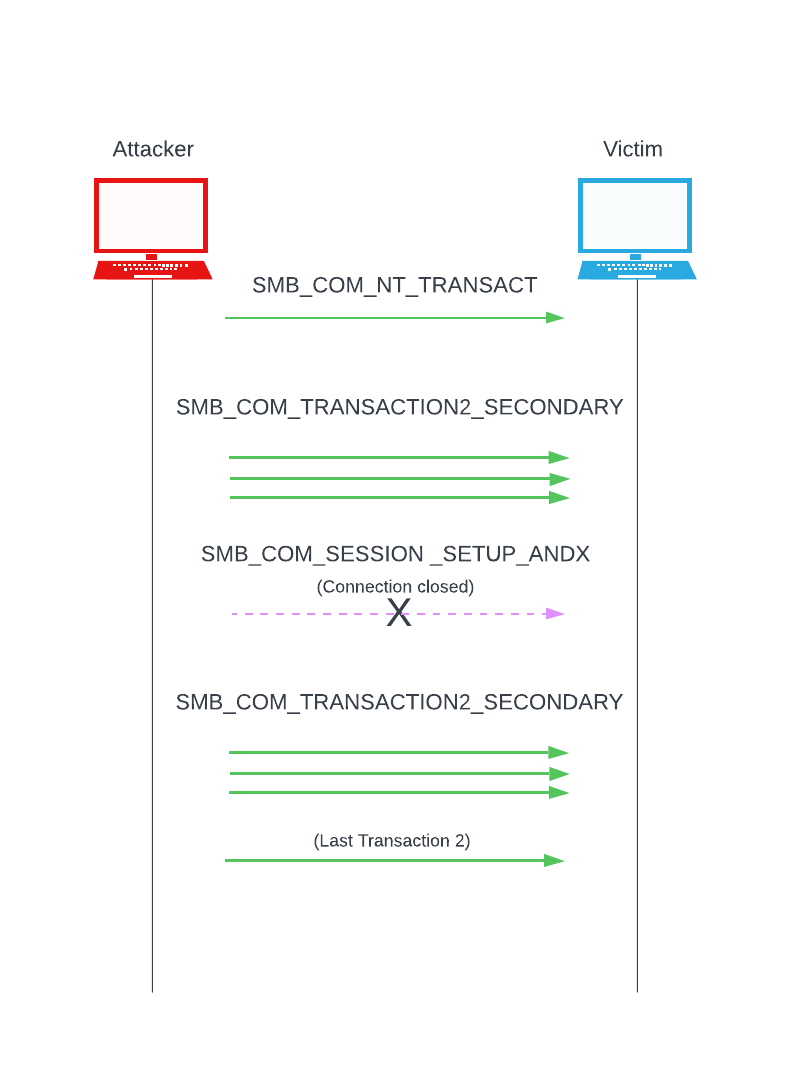
\includegraphics[scale=0.5]{images/exploit_5_comm.png}
      \caption{Buffer overflow - communications}
\end{figure}

\begin{figure}[ht!]
    \centering
      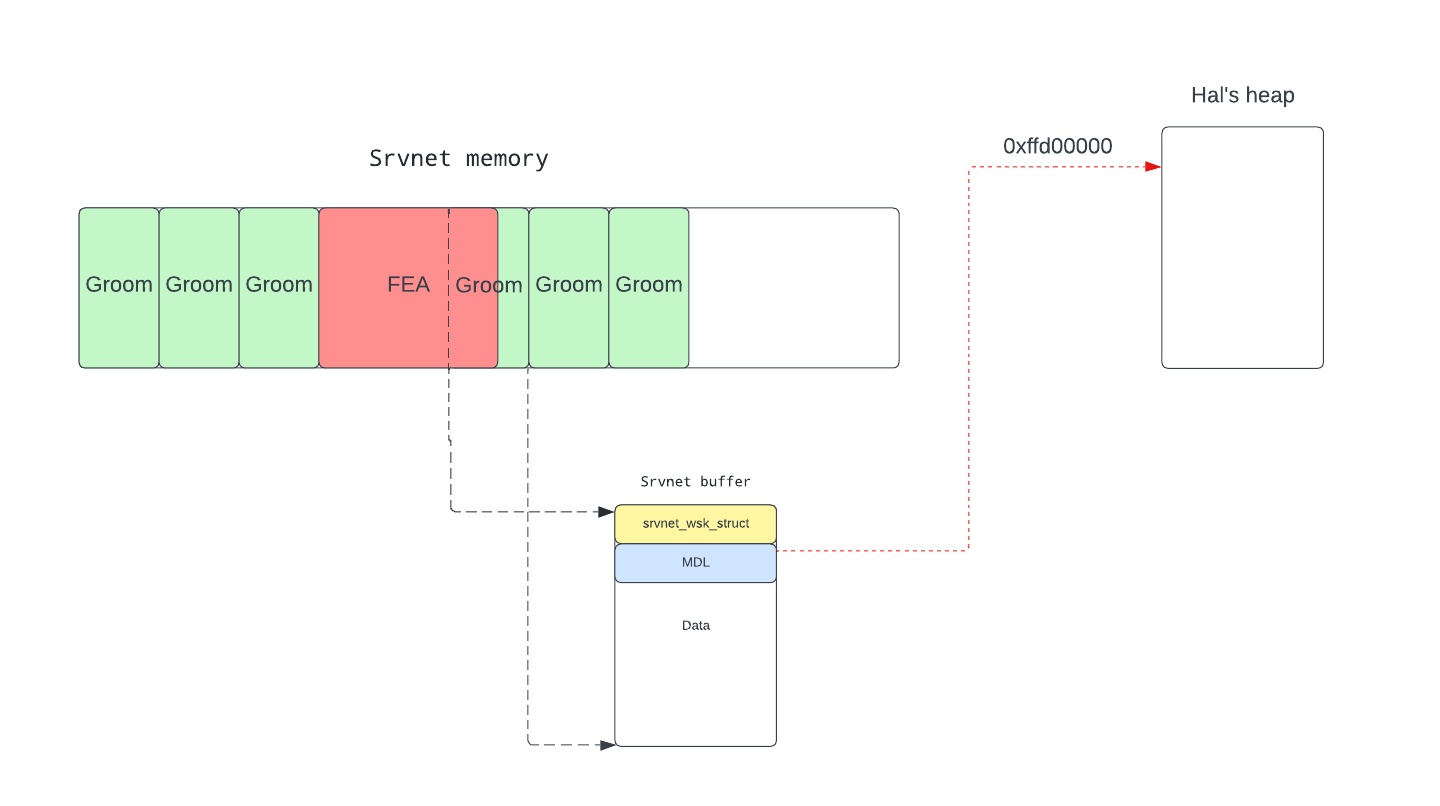
\includegraphics[scale=0.5]{images/exploit_5_buff.png}
      \caption{Buffer overflow - memory buffer}
\end{figure}

\clearpage
\subsection{Payload injection}
At this point, the data of the next transaction will not be stored in the srvnet buffer because the MDL points to the HAL's heap.\\
So, the attacker sends the payload, which is the DoublePulsar shellcode and a function handler, in the next transaction data.
Now the attacker has memorized his payload in the HAL's heap.

\begin{figure}[ht!]
    \centering
      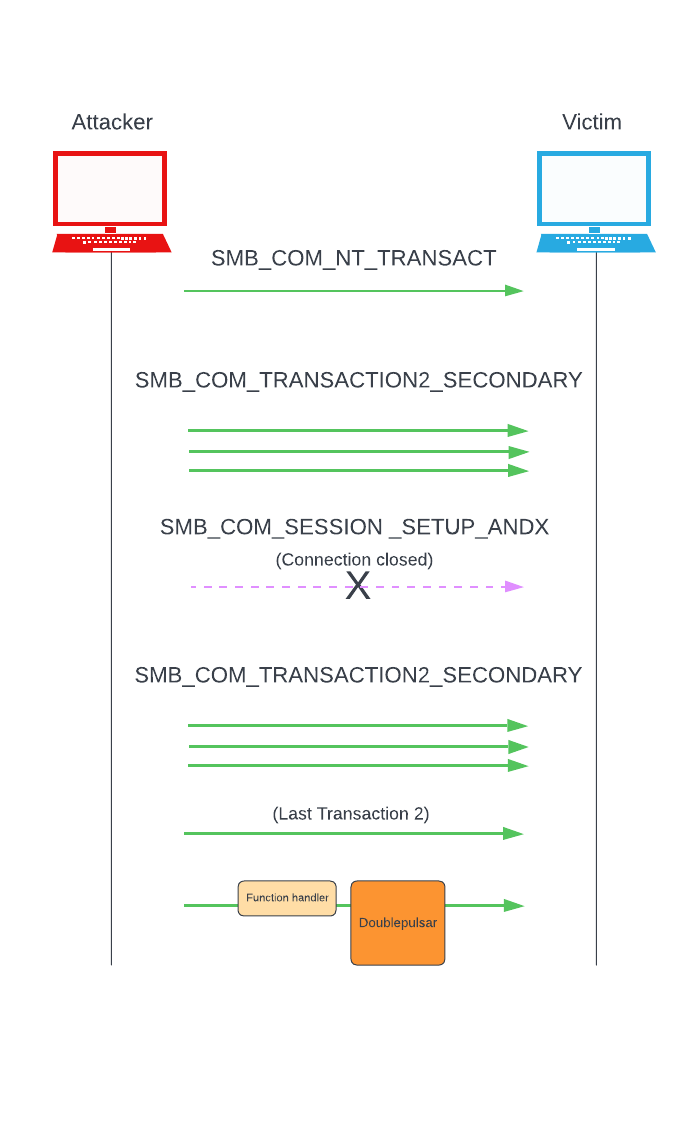
\includegraphics[scale=0.5]{images/exploit_6_comm.png}
      \caption{Payload injection - communications}
\end{figure}

\begin{figure}[ht!]
    \centering
      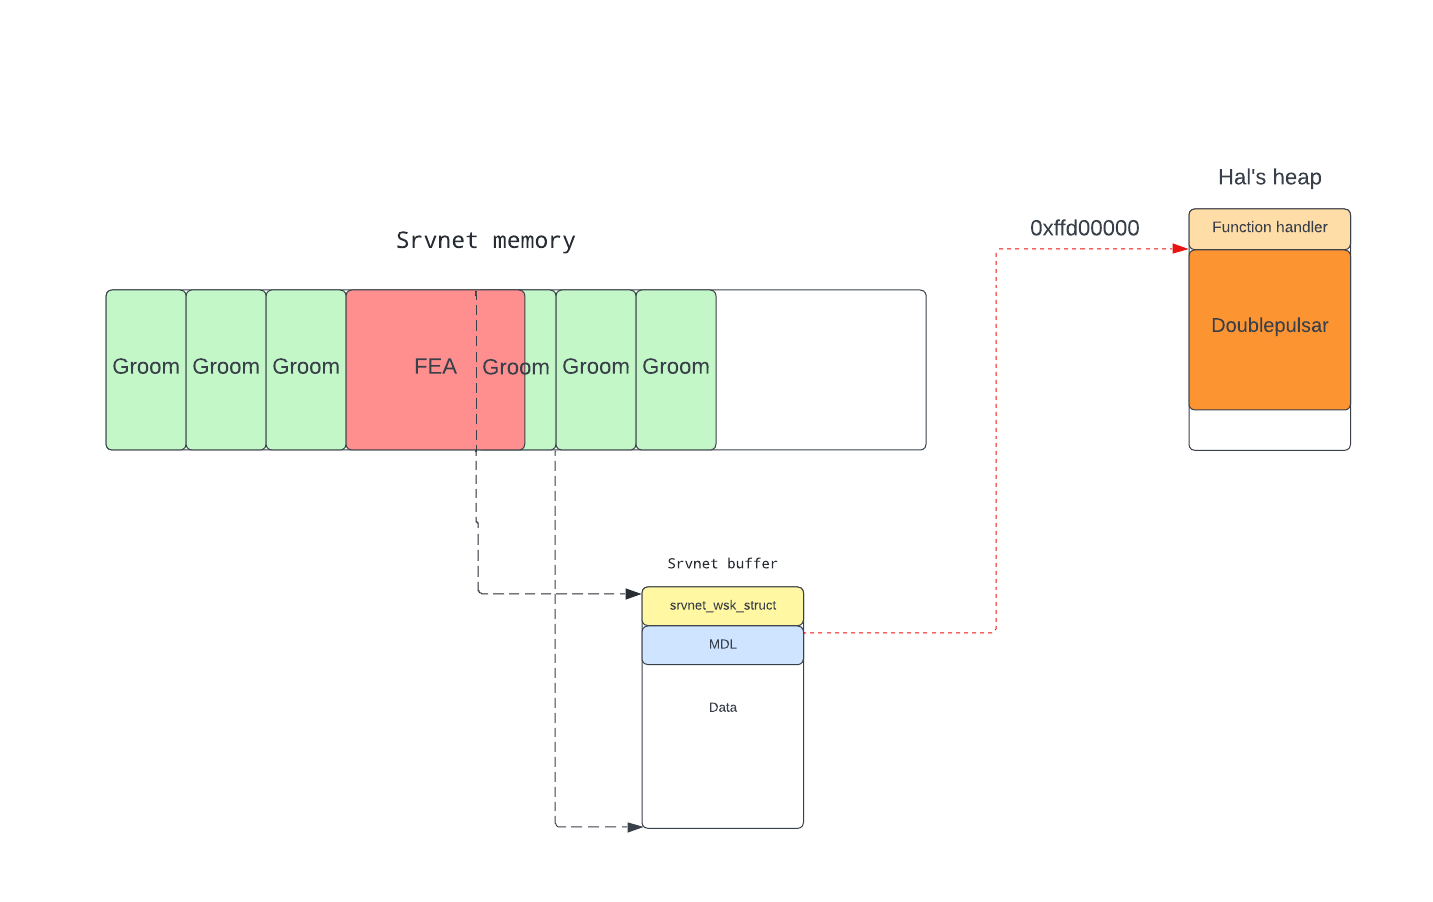
\includegraphics[scale=0.5]{images/exploit_6_buff.png}
      \caption{Payload injection - memory buffer}
\end{figure}

\clearpage
\subsection{Remote code execution}
In this last point the attacker wants to execute the DoublePulsar shellcode in the HAL's heap.\\
To do that the attacker closes all the auxiliary connection, this will trigger the function SrvNetWskReceiveComplete() for each memory allocation.\\
For the srvnet buffer that he has overflowed the pointer of the SrvNetWskReceiveComplete() points to the function handler in the HAL's heap. 
When the function handler is triggered it executes the DoublePulsar shellcode with root permissions.\\
The attacker has successfully executed the payload on the Windows server and he has the complete control of it.

\begin{figure}[ht!]
    \centering
      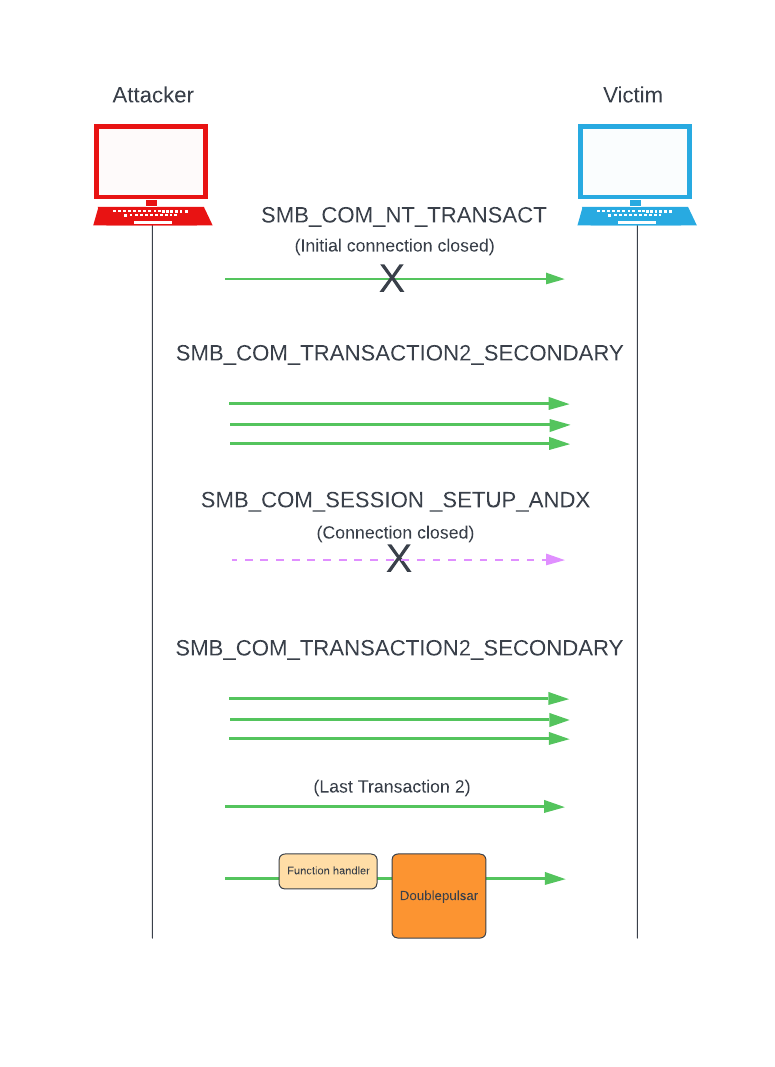
\includegraphics[scale=0.5]{images/exploit_7_comm.png}
      \caption{Remote code execution - communications}
\end{figure}

\begin{figure}[ht!]
    \centering
      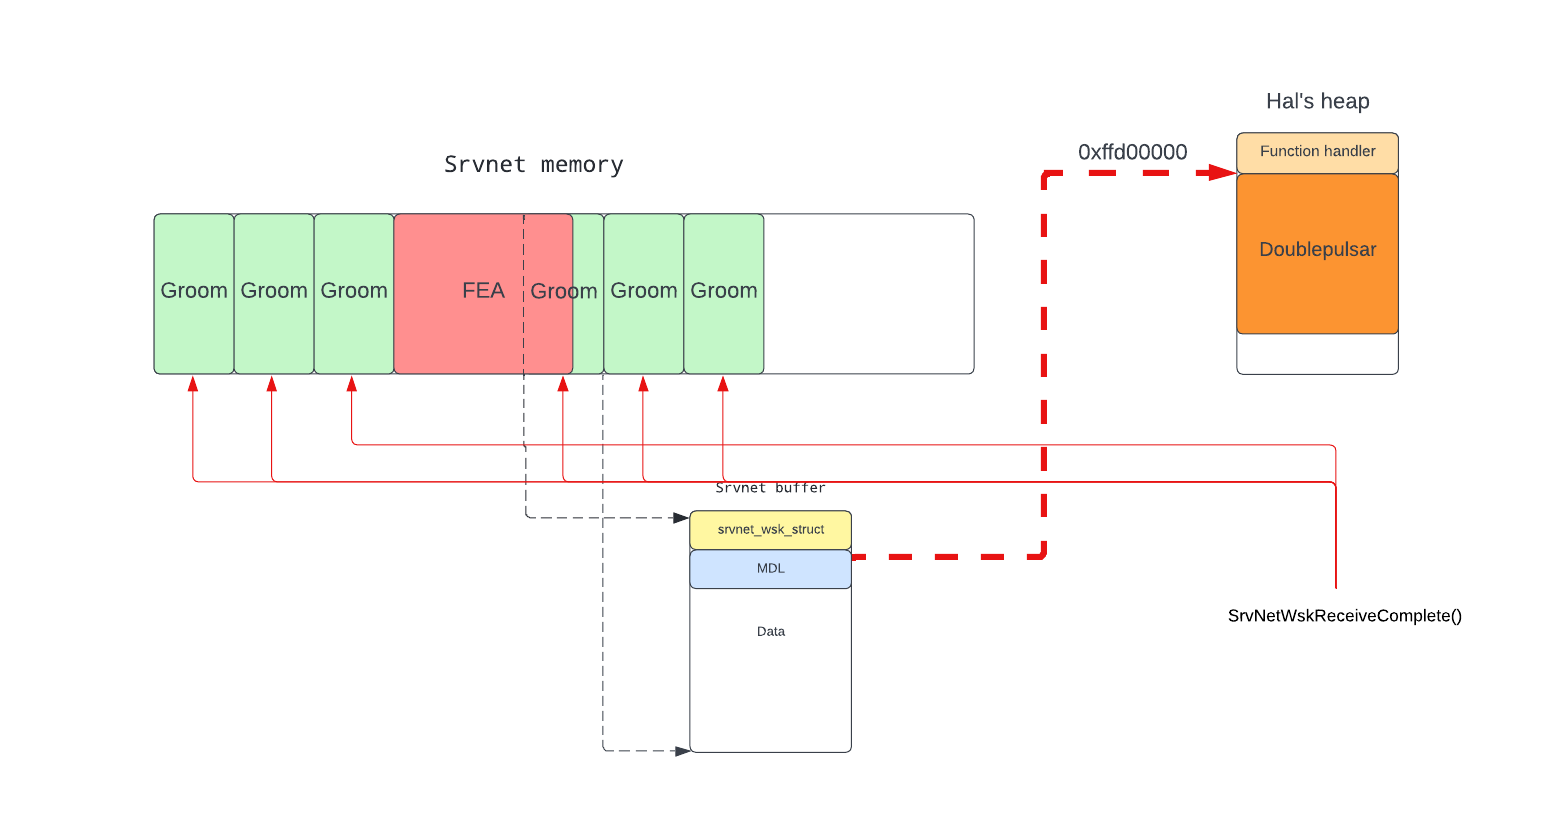
\includegraphics[scale=0.5]{images/exploit_7_buff.png}
      \caption{Remote code execution - memory buffer}
\end{figure}